\thispagestyle{plain}
\newpage
\section{Requirement Capture and Analysis}\label{sec:requirement-capture}

\normalsize

According to~\citet{anton2003successful}: \textquote{good requirements planning means software can be cheaper to produce, easier to build, and less prone to unexpected failure.}
Requirements for this project considered the business, user, and functional requirements in different scenarios where the product might be used~\citep{wiegers2000karl, potts1994inquiry}.
The requirement specification additionally considered the different types of people who would be using the product.
It is the combination of the gathered requirements that informs the product's design.

\subsection{The Case For Business}\label{subsec:the-business-case}

\citet{wiegers_hokanson_2023} state in their new book that enterprise software product requirements~\gls{stem} from the core business requirements.
These business requirements inform resultant system, user, and solution requirements.
See Figure~\ref{fig:requirements-diagram} for Wiegers' and Hokanson's representation of this influence.
In addition, due to the nature of enterprise, certain business rules and constraints will influence the solution requirements.
\gls{sie}'s PlayStation is a high-profile brand, so additional considerations must be taken when operating in this space.
See Table~\ref{tab:business-requirements} for the business requirements that help inform the other requirements of the project.

\begin{figure}[!htb]
    \minipage{\textwidth}
    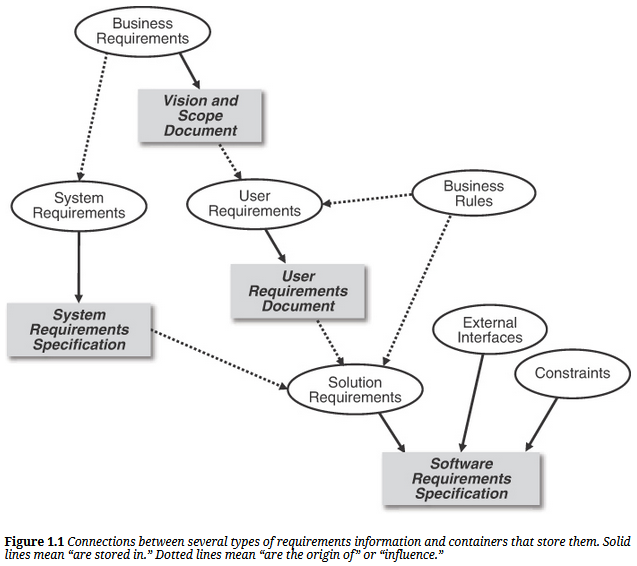
\includegraphics[width=\linewidth]{requirements-diagram}
    \caption{Taken from~\citep{wiegers_hokanson_2023}}\label{fig:requirements-diagram}
    \endminipage\hfill
\end{figure}

\begin{tabularx}{\textwidth}{szs}
    \caption{Business Requirements}\label{tab:business-requirements}\\
    \toprule
    \textbf{Code} & \textbf{Business Requirement} \\\midrule
    B1 & Increase the accessibility to spatial audio technology for~\glspl{pspartner} \\\midrule
    B2 & Inform~\glspl{pspartner} and potential~\glspl{pspartner} of the nature and capabilities of spatial audio \\\midrule
    B3 & Increase the engagement of~\glspl{pspartner} with PlayStation's platform \\\midrule
    B4 & Demonstrate how spatial audio relates to the interests of~\glspl{pspartner} \\\midrule
    B5 & Increase the availability and flexibility of~\gls{sie}'s technical services \\\bottomrule
\end{tabularx}

\subsection{System Requirements}\label{subsec:system-requirements}
The problem statement in~\ref{subsec:problem-statement} makes things easy for the formulation of the key \textit{system} requirements\footnote{\citet{wiegers_hokanson_2023} define system requirements as: \textquote{A description of a top-level capability or characteristic of a complex system that has multiple subsystems, often including both hardware and software elements.}} for this system.
This project defines the~\gls{mvp} in terms of the minimal functionality the system must have in order for the project to be considered successful.
These requirements can be found in Table~\ref{tab:system-requirements} and cover the technical requirements for the solution in relation to the business requirement.

\begin{tabularx}{\textwidth}{szs}
    \caption{System Requirements}\label{tab:system-requirements}\\
    \toprule
    \textbf{Code} & \textbf{System Requirement} & \textbf{Business Requirement Code (s)} \\\midrule
    S1 & The system shall be accessible to the user through the use of a standard internet browser & B1 \\\midrule
    S2 & The system shall allow the user to upload their own audio file & B2, B3 \\\midrule
    S3 & The system shall separate the uploaded audio file into its constituent instrument~\glspl{stem} & B2 \\\midrule
    S4 & The system shall provide the means for the user to define spatial parameters for each~\gls{stem} & B2, B3 \\\midrule
    S5 & The system shall render a spatial audio file taking the instrument~\glspl{stem} and the user-defined spatial parameters as input & B2 \\\midrule
    S6 & The system shall deliver the rendered audio file to the user through the web browser & B1, B2 \\\midrule
    S7 & The system shall exist entirely within the~\gls{aws} public cloud ecosystem & B1, B5 \\\midrule
    S8 & The system shall use~\glspl{hrtf} to render spatial audio, mimicking the functionality of the~\gls{tempest_3d_audio} & B2, B4, B5 \\\bottomrule
\end{tabularx}

\subsection{User Requirements}\label{subsec:user-requirements}
The functional needs of the system are simple to pin down, however, the user requirements require slightly more nuance.
The concept of `user stories' has faced criticism in the literature for over-focus towards the `story', rather than the `user' and their role~\citep{hudson2013user}.
\citet{hudson2013user} highlights `persona stories' as an alternative that takes into account the nature of the user: we ask ourselves the question: ``what does this person, in this role, require from the system?''

\subsubsection{Dramatis Personae}
Three personae were formulated as potential users of the project, each with their own background and motivations:

\begin{enumerate}
    \item Game Developer\textemdash wants to develop a game using spatial audio\textemdash they not yet onboarded with PlayStation partners, and want to see a demonstration of what the PlayStation platform can offer in terms of its spatial audio capabilities\textemdash this will inform their future choice of development platform.
    \item Audio Enthusiast\textemdash has prior experience with stereo audio\textemdash wants to experience spatial audio applied to their favorite song.
    \item Novice\textemdash stumbled across the feature\textemdash no prior experience of spatial audio or even game development\textemdash likes immersive media experience so feels an interest towards the concept of spatial audio.
\end{enumerate}

The user requirements were formulated with these three personae in mind.
The product is intended to be a customer-facing one so consideration towards a wide range of potential customers were considered.

\begin{tabularx}{\textwidth}{szzs}
    \caption{User Requirements}\label{tab:user-requirements}\\
    \toprule
    \textbf{Code} & \textbf{User Requirement} & \textbf{Persona (e) Addressed} & \textbf{Business Requirement Code (s)} \\\midrule
    U1 & The user shall be able to understand and use the system easily & Novice & B1 \\\midrule
    U2 & The system shall have high-quality audio rendering quality & Game Developer, Audio Enthusiast & B2, B4 \\\midrule
    U3 & The user shall be informed by using the system & Novice, Game Developer & B1, B4 \\\midrule
    U4 & The system shall be easier set up and run than a local environment & Game Developer & B1, B5 \\\midrule
    U5 & The system pipeline shall complete quickly & Novice, Audio Enthusiast, Game Developer & B3, B5 \\\bottomrule
\end{tabularx}

\subsection{Business Rules\ldots OK?}\label{subsec:business-rules-ok}

Finally, the system's design must also take into account the operation of~\gls{sie} as a company in its design:

\begin{itemize}
    \item The proprietary spatialisation software that is used by the~\gls{ps5} is a company secret, therefore the system should not use it in this prototype.
    \item \gls{sie} is concerned with being profitable, therefore costs should be minimised in the development and running of the service.
    \item The creation of the prototype should not be done in the~\gls{sie}~\gls{aws} environment.
    \item \gls{sie} retains tight control over the PlayStation~\gls{ip} therefore its branding should not be present in the prototype.
\end{itemize}

These business rules will inform the design and the development practises of the project, particularly in relation to security and cost management.